\section{Box inside the Boat}
The boat should be waterproof. However, there should be a second waterproofing layer. Therefore, two boxes were made for the insides 
of the boat. They were laser cut from acrylic 3 mm, connected with 3D printed with PLA brackets \autoref{Figure: bracket 15x15 CAD design}, 
and then the connection between the parts was filled with silicon \autoref{Figure: Box silicon}. 
%maybe here about the frames
\begin{figure}[H]
    \centering
    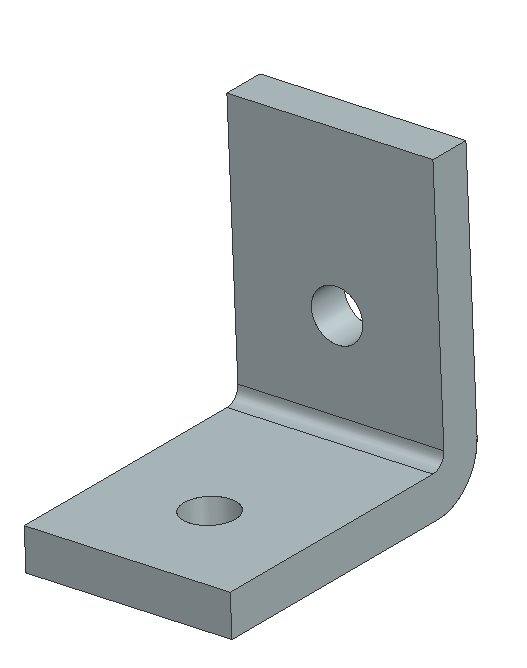
\includegraphics[width=0.4\textwidth]{bracket_1.png}
    \caption{Bracket 15x15 CAD Design}
    \label{Figure: bracket 15x15 CAD design}
\end{figure} 
\begin{figure}[H]
    \centering
    \begin{subfigure}[b]{0.4\textwidth}
        \centering
        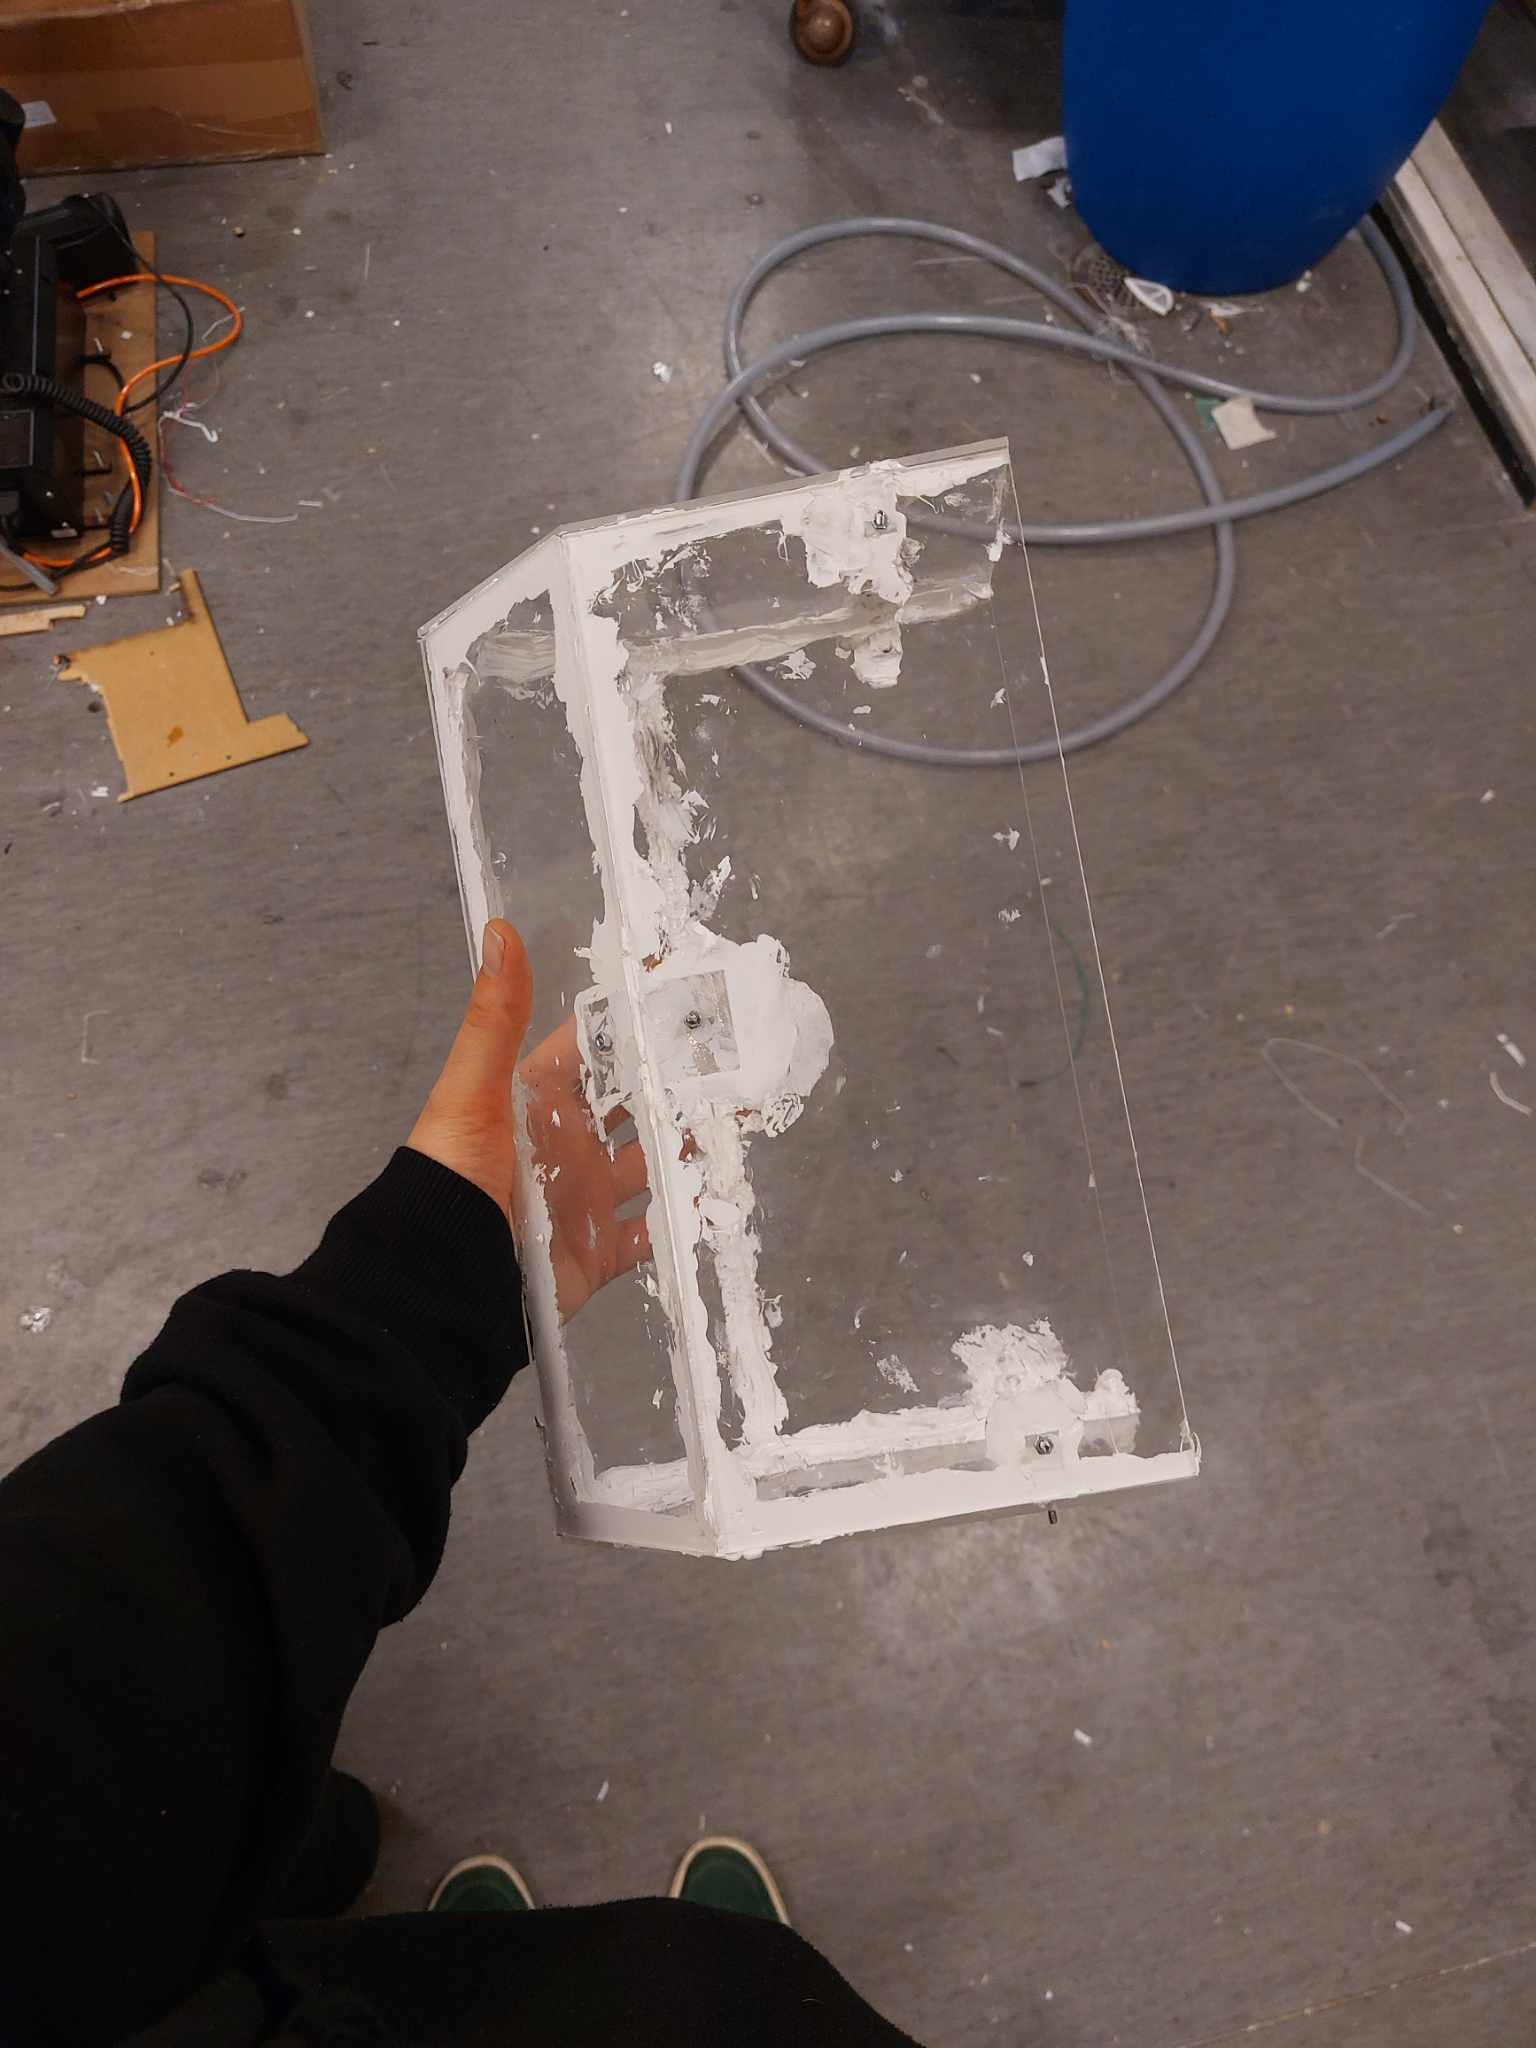
\includegraphics[width=\textwidth]{box_silicon_1.jpg}
    \end{subfigure}
    \begin{subfigure}[b]{0.4\textwidth}
        \centering
        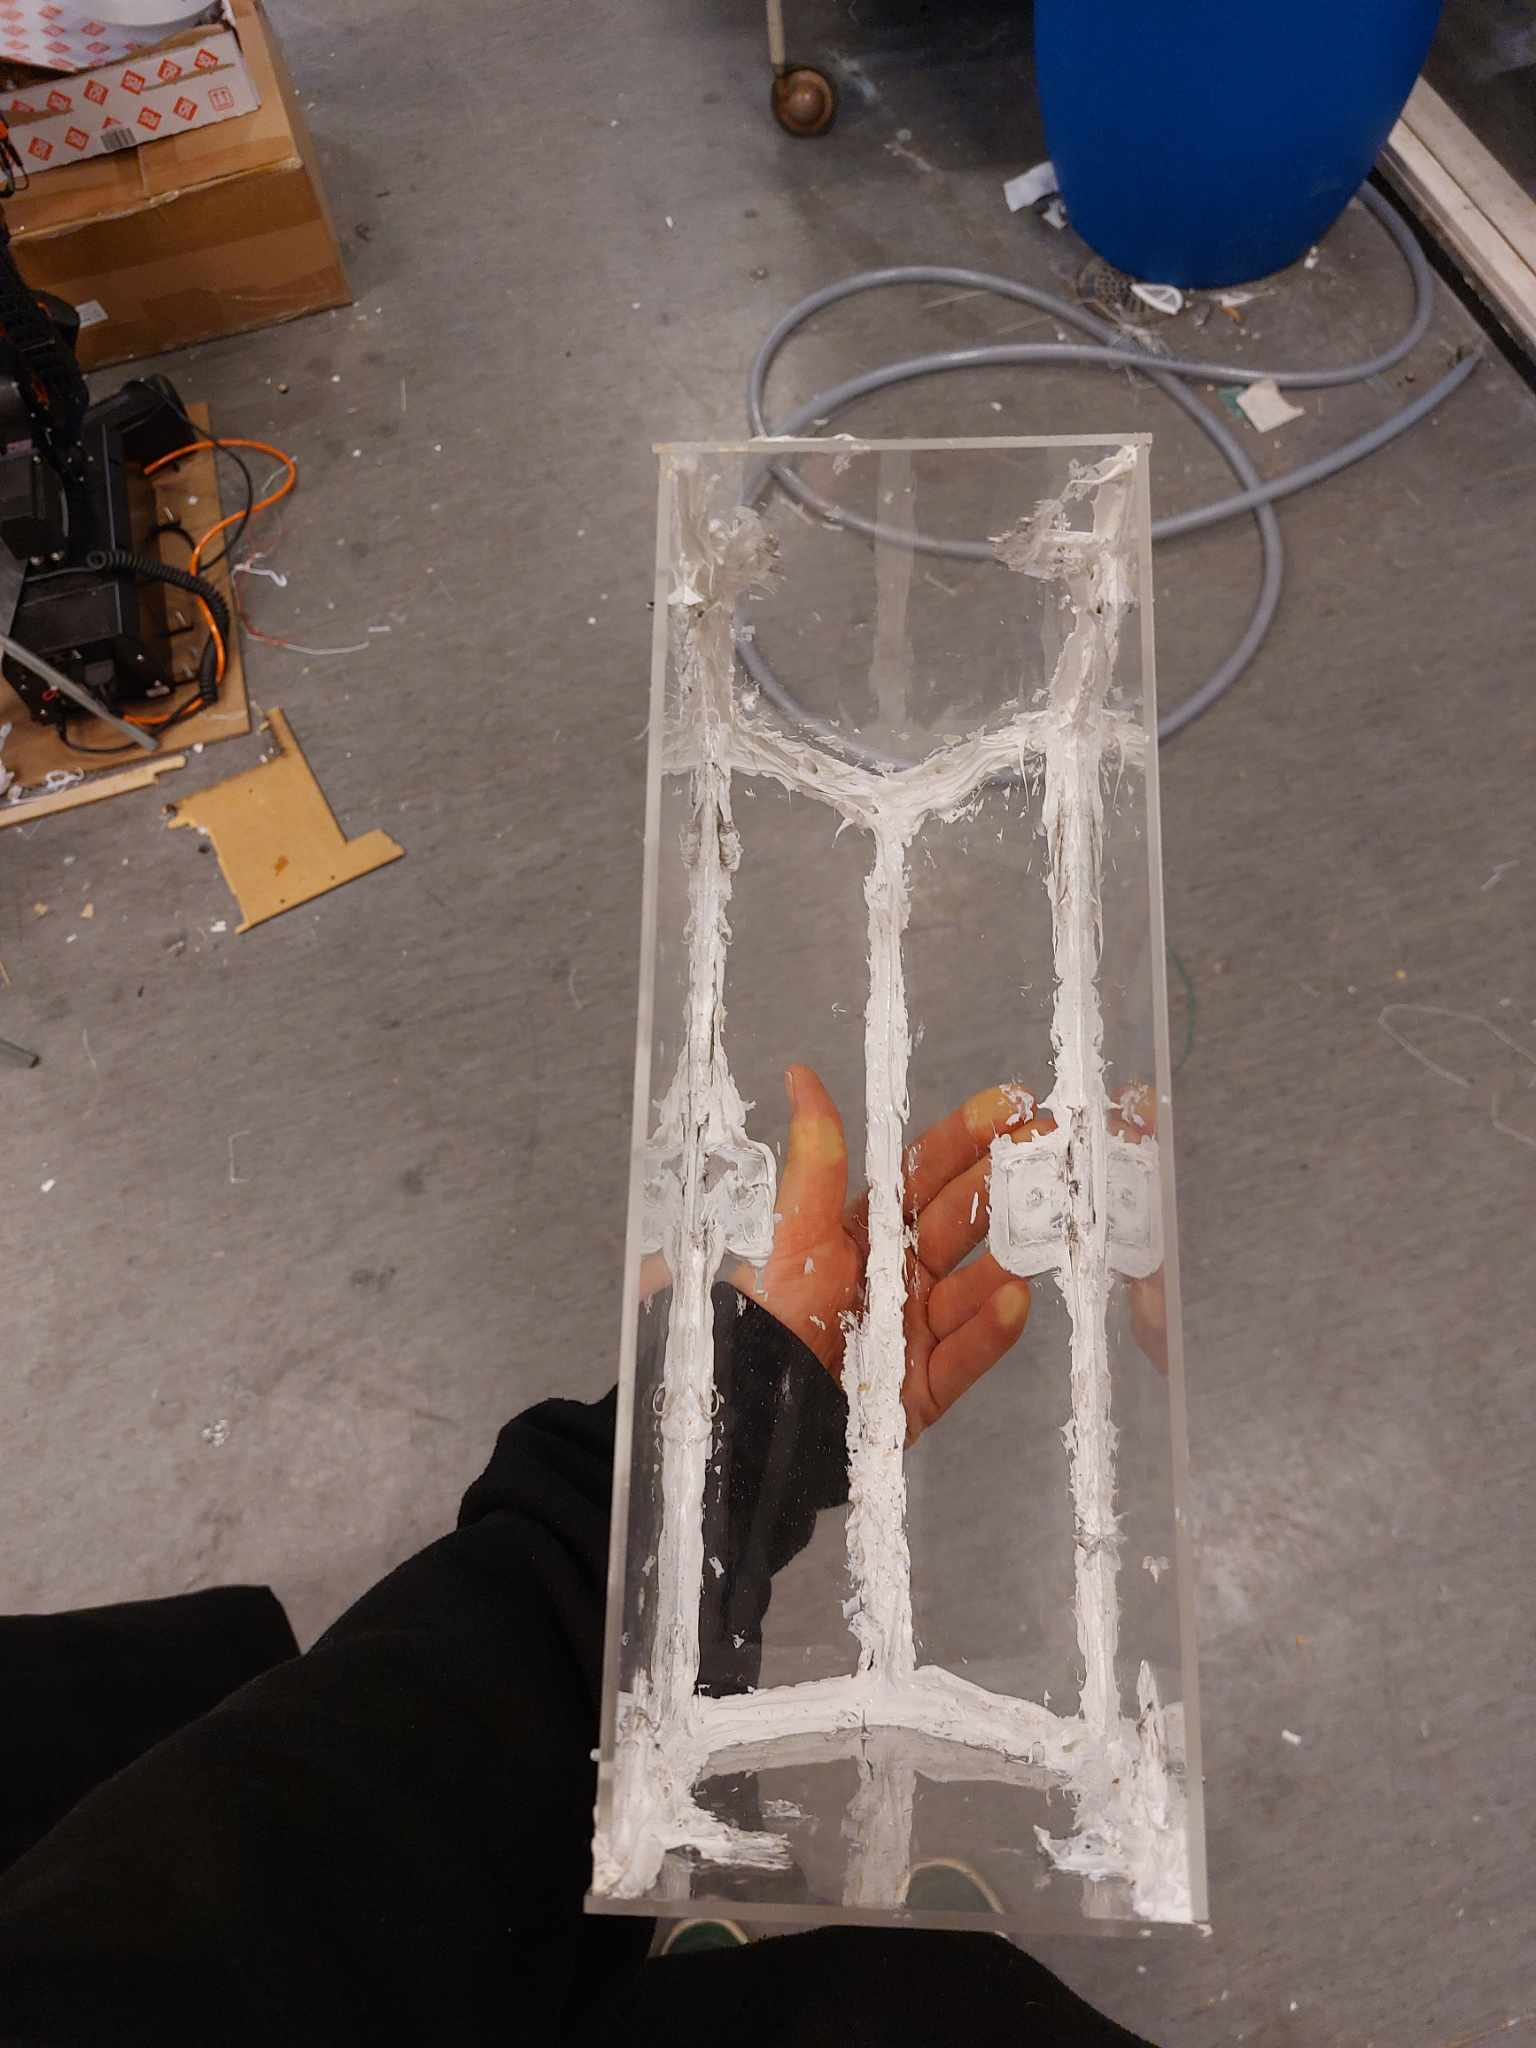
\includegraphics[width=\textwidth]{box_silicon_2.jpg}
    \end{subfigure}
       \caption{Box with Silicon}
       \label{Figure: Box silicon}
\end{figure}
The top of the boxes had two versions. Version one \autoref{Figure: Version 1 of the Box} was supposed be stuck on the bottom part. However, 
after testing it turned out it would not secure the components from the water when it was flipped. 
\begin{figure}[H]
    \centering
    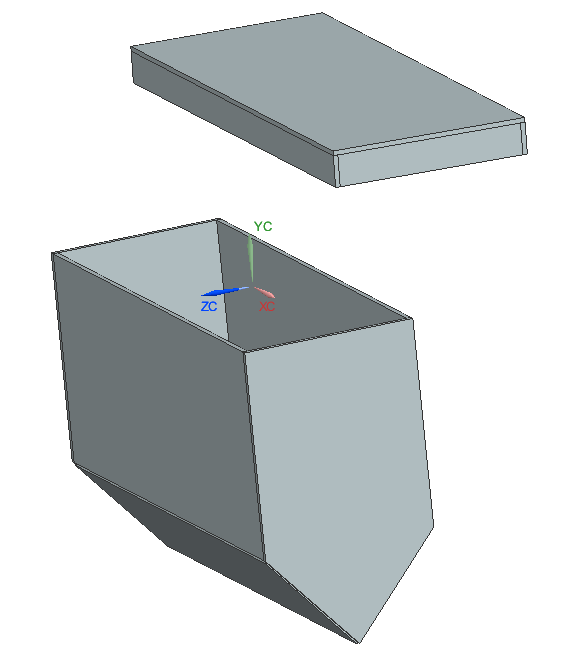
\includegraphics[width=0.4\textwidth]{box_1.png}
    \caption{Version 1 of the Box}
    \label{Figure: Version 1 of the Box}
\end{figure} 
Therefore, the version number two \autoref{Figure: Version 2 of the Box} was designed. It was designed to be a plain rectangle 
screwed to the 3D printed frames. The frame is a tight fit to the box, and the top plate is screwed into the 3D printed from PLA frame.
\begin{figure}[H]
    \centering
    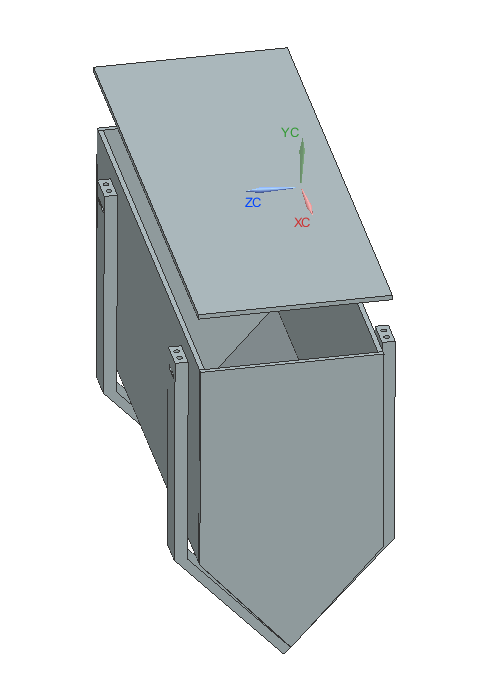
\includegraphics[width=0.4\textwidth]{box_3.png}
    \caption{Version 2 of the Box}
    \label{Figure: Version 2 of the Box}
\end{figure} 

Inside each box there has to be a battery. In one of the boxes there have to be rest of the electrical components. To fit the battery and tower 
inside the boat, two plates were laser cut from 5 mm MDF. They will be put in both boxes and prevent components from moving. \\
\begin{figure}[H]
    \centering
    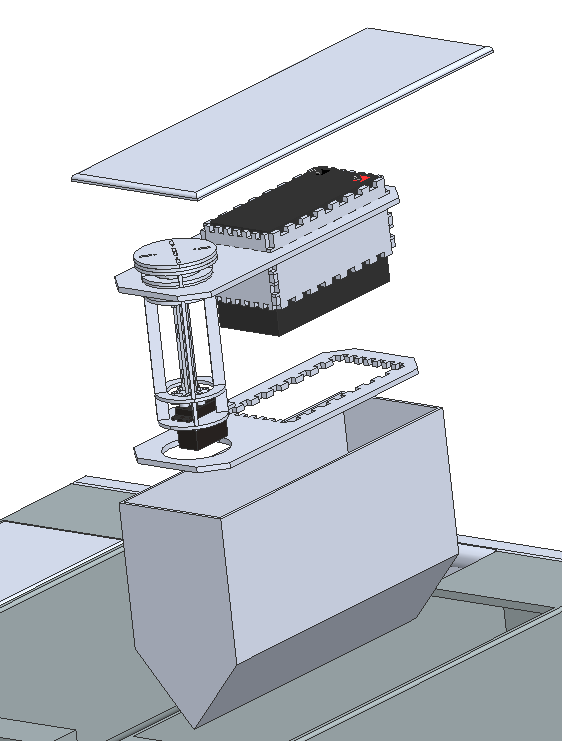
\includegraphics[width=0.4\textwidth]{box_2.png}
    \caption{One of the Boxes with Inside}
    \label{Figure: One of the boxes}
\end{figure} 
One of the boxes, while testing the waterproofing, started leaking. The second one did not, even though both of them were done the same. 
Therefore, one of the boxes had to be done from the beggining. Afterwards, it was tested again and the test was successful. 
